\documentclass[revtex4-2]{mpltx}
\usepackage{physics}

\begin{document}
\title{NaI (Tl) 闪烁谱仪测定 $\gamma$ 射线能谱}
\author{方尤乐}

\emailphone{eden@stu.pku.edu.cn}{(86)15313960363}
\affiliation{北京大学物理学院\quad 学号: 2000012416}
\begin{abstract}
    本实验利用 NaI (Tl) 闪烁谱仪,探讨和研究了闪烁体探测器的基本工作原理,以及 $\gamma$ 射线与物质相互作用的基本规律。
    实验中首先通过示波器观察 NaI (Tl) 闪烁体探头探测的脉冲图形,
    然后利用单道脉冲幅度分析器采集了 137Cs 源的 $\gamma$ 全能谱,
    随后结合 137Cs 源和 60Co 源的峰位对谱仪进行了能量刻度;
    在此基础上,利用多道分析器再次获得了 60Co、137Cs 源的全能谱,进一步测定了 137Cs,60Co 的混合能谱,对结果进行了分析比较和讨论。
\end{abstract}
\keywords{闪烁谱仪,能谱,$\gamma$ 射线,多道分析器}
\maketitle
\section{引言}
    闪烁体探测器是利用某些物质在射线作用下会发光的特性来探测射线的仪
    器;它的主要优点是,既能探测各种类型的带电粒子,又能探测中性粒子,既能探测粒子强度,又能探测粒子能量;并且探测效率高,分辨时间短。
    它在核物理研究和放射性同位素的测量中得到了广泛的应用。
    本实验的目的是了解闪烁谱仪的原理、特性、结构,掌握闪烁谱仪的使用方法,鉴定它的能量分辨率和能量线性关系,
    并通过测定 137Cs,60Co  $\gamma$ 射线的能谱。了解 $\gamma$ 射线与物质相互作用的基本规律。
\section{实验装置}
    NaI (Tl) 闪烁谱仪由闪烁体探头(含光电倍增管)和后端仪器组成。
    电压信号经进一步线性放大后,可由示波器显示脉冲波形,
    也可以输入单道分析器进行脉冲幅度分析和统计,
    或者输入微机多道分析器自动获得射线的能谱。
    
    \begin{figure}[htbp]
        \centering
        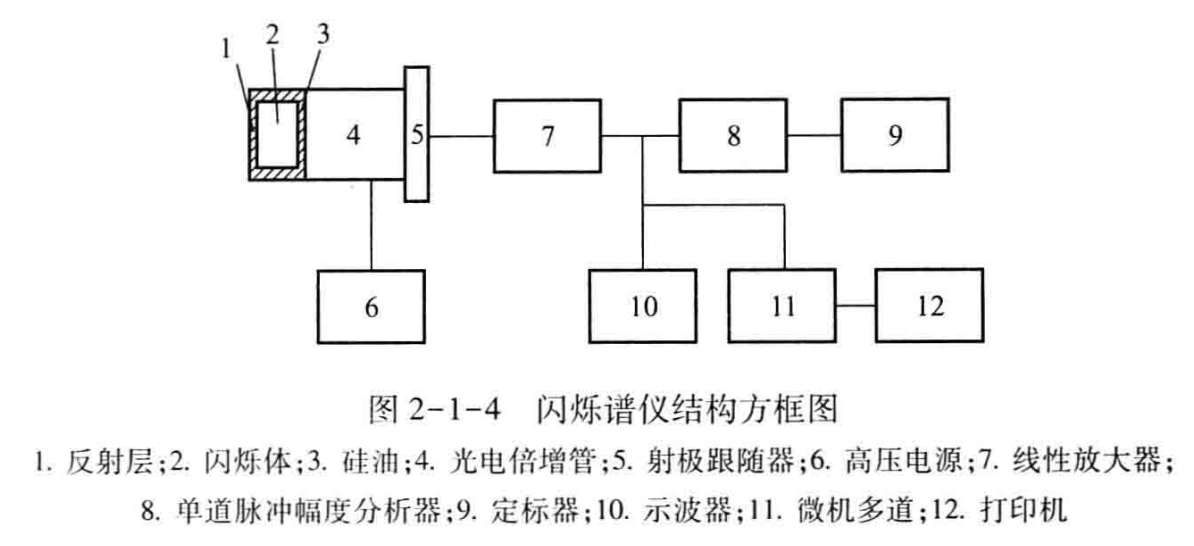
\includegraphics[width=0.8\textwidth]{./pic0.png}
        \caption{NaI (Tl) 闪烁谱仪示意图}\label{fig:0}
    \end{figure}

    其中单道分析器只容许 $V\sim V + \Delta V$ 幅度的脉冲通过,
    可以调节阈值 V 和道宽 $\Delta V$,
    并可以在一个固定时间间隔内(本实验设置为 30 秒)对通过的脉冲数量进行统计;
    微机多道分析器则可以同时对一定范围内的所有脉冲间隔 $V_x \sim V_{x+1}=V_x+\Delta V$ 进行监测计数,
    x 为道址,由此可极大提高效率,本实验采用微机多道分析器时。
\section{结果与分析}
    \subsection{单道测量}
    首先利用单道逐点计数测定 137Cs 的能谱。调节放大倍数为 28.48,测量 30 秒
    固定道宽 0.1 V, 结果如下:
    \begin{figure}[htbp]
        \centering
        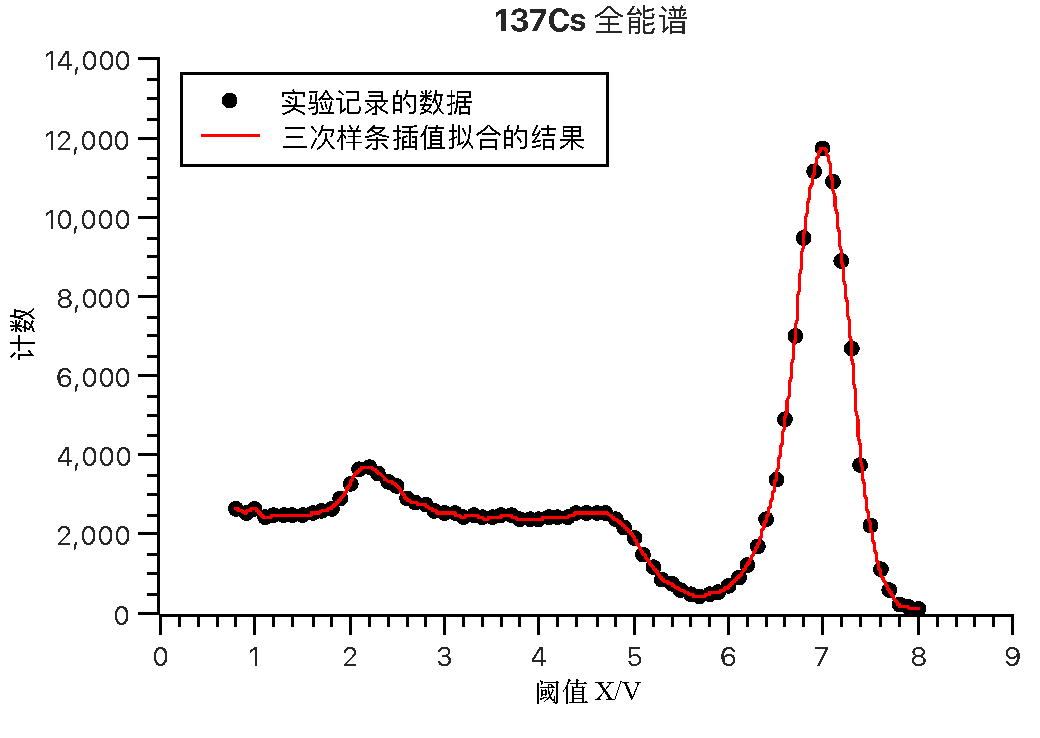
\includegraphics[width=0.8\textwidth]{./pic1.pdf}
        \caption{137Cs 全能谱}
    \end{figure}

    可以观测到137Cs 的全能峰 0.662 MeV 和反散射峰 0.184MeV。
    137Cs 只放出单一能量的 0.662MeV $\gamma$ 射线,它与NaI晶体
    的相互作用只包含光电效应和康普顿散射。
    图中全能峰左侧的平台是来自于康普顿电子的贡献。部分入射的 $\gamma$ 射线穿过 NaI 晶体打到光电倍增管上
    发生 180度的康普顿散射,反散射的光子返回时再次与晶体发生光电效应,由此形成了 0.184MeV 的反散射峰。

    可以估计 137Cs 的两个特征峰值对应的阈值,$0.184$ MeV 对应单道阈值 $2.17$V, 
    $0.662$ MeV 对应单道阈值 $6.97$V。利用 137Cs 谱的全能峰估计谱仪的能量分辨率:
    \begin{align*}
        &\Delta E=(7.32-6.65)\mathrm{V} = 0.67\mathrm{V}\\
        &E_0 = 6.97 \mathrm{V}\\
        &\epsilon=\frac{\Delta E}{E_0} = \frac{0.67}{6.97} 
        = 0.096
    \end{align*}

    \subsection{对闪烁体谱仪做能量刻度}
    由于调节电压阈值的量程有限,为了能测量和利用 60 Co 的特征峰值进行标定,将放大系数降低到
    原来的一半,即 14.24,在 137Cs 和 60Co 的特征峰附近进行单道计数,对每个阈值测量 30 秒进行计数,结果如\autoref{fig:1}。
    \begin{figure}[htbp]
        \centering
        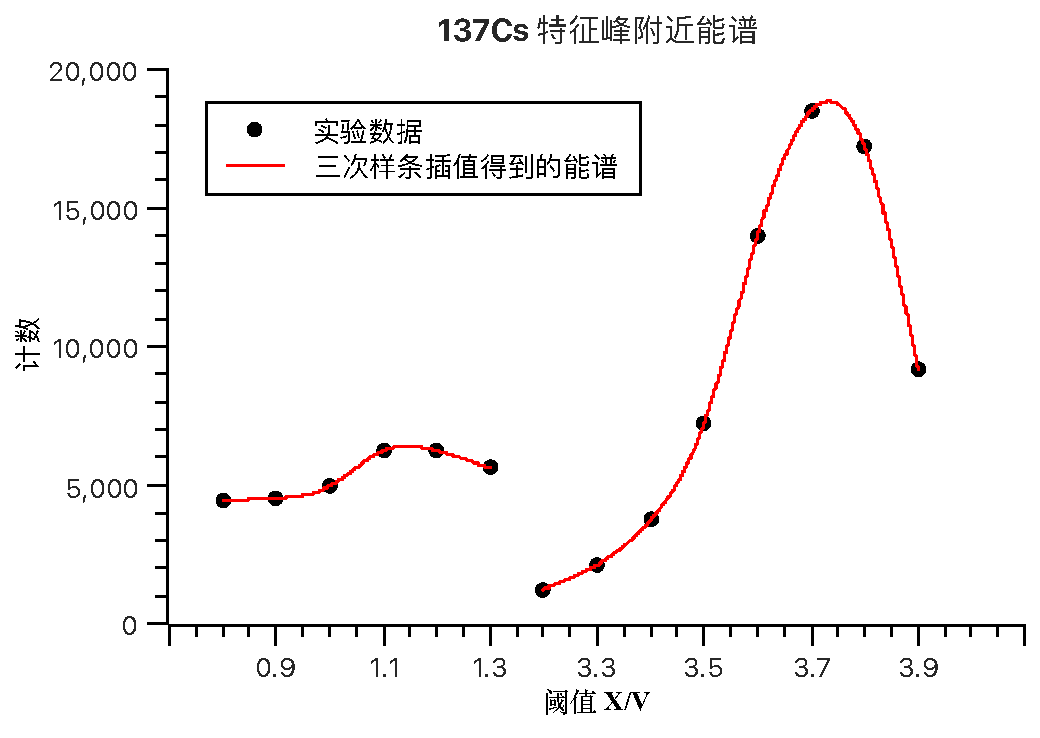
\includegraphics[width=0.5\textwidth]{./pic3.pdf}
        \caption{137Cs 两个特征峰附近的能谱}\label{fig:1}
    \end{figure}

    再对 60Co 源的两个特征峰值附近进行单道计数,结果如\autoref{fig:2}。
    \begin{figure}[htbp]
        \centering
        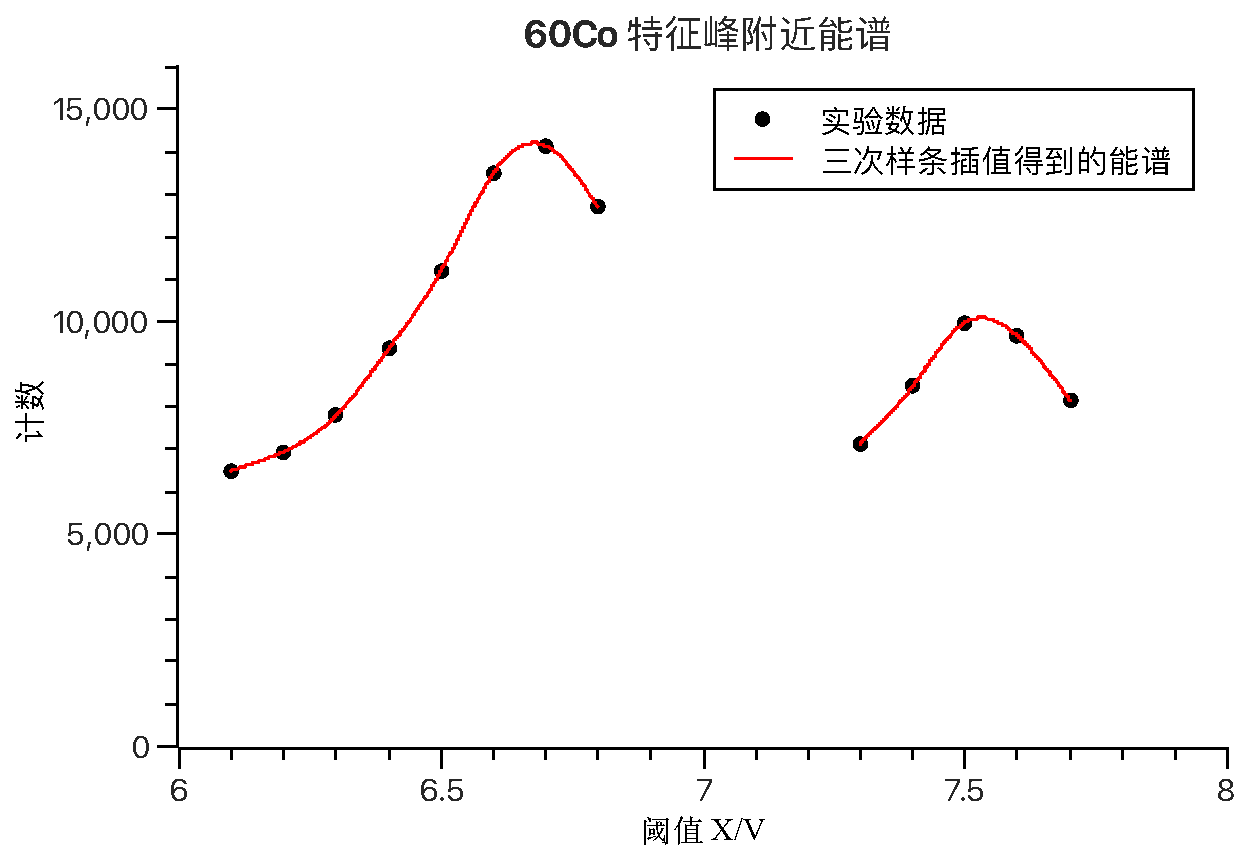
\includegraphics[width=0.5\textwidth]{./pic2.pdf}
        \caption{60Co 特征峰值附近能谱}\label{fig:2}
    \end{figure}

    得到 $0.662$ MeV 对应 单道阈值 $3.73$V,$0.184$ MeV 对应 $1.15$V。
     $1.33$ MeV 对应 $7.53$V, $1.17$ MeV 对应 $6.68$V。
    因此可以对四个数据进行线性拟合得到阈值和能量的关系:见\autoref{fig:3}。
    \begin{figure}[htbp]
        \centering
        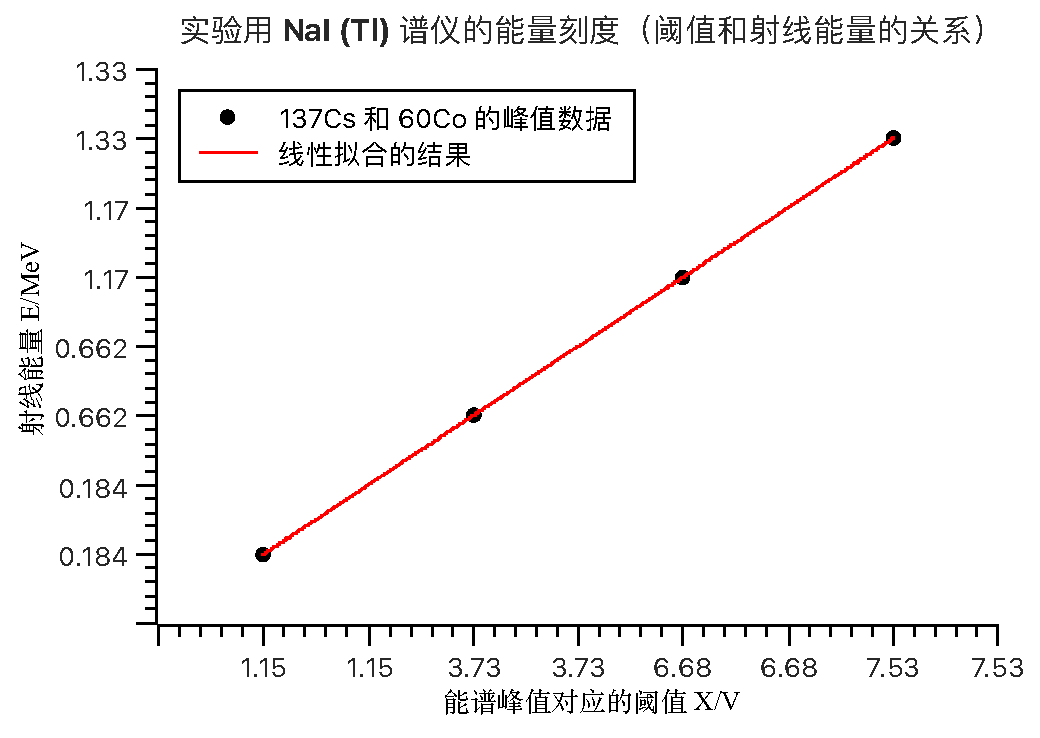
\includegraphics[width=0.5\textwidth]{./pic4.pdf}
        \caption{实验用 NaI (Tl) 谱仪的能量刻度(阈值和能量的关系)}\label{fig:3}
    \end{figure}
    相关系数为 0.99986,因此阈值和能量之间存在较好的线性关系,
    并由此得到 NaI (Tl) 谱仪的能量刻度:
    \begin{equation}
        E/\mathrm{MeV} = 0.1785 X/\mathrm{V} - 0.0153
    \end{equation}

    \subsection{使用微机多道分析器}
    改变放大倍数至 10.4,用微机多道探测器进行测量,时限设为 5 分钟。得到的 137Cs 能谱如\autoref{fig:5},
    60Co 能谱如\autoref{fig:6}。
    \begin{figure}[htbp]
        \centering
        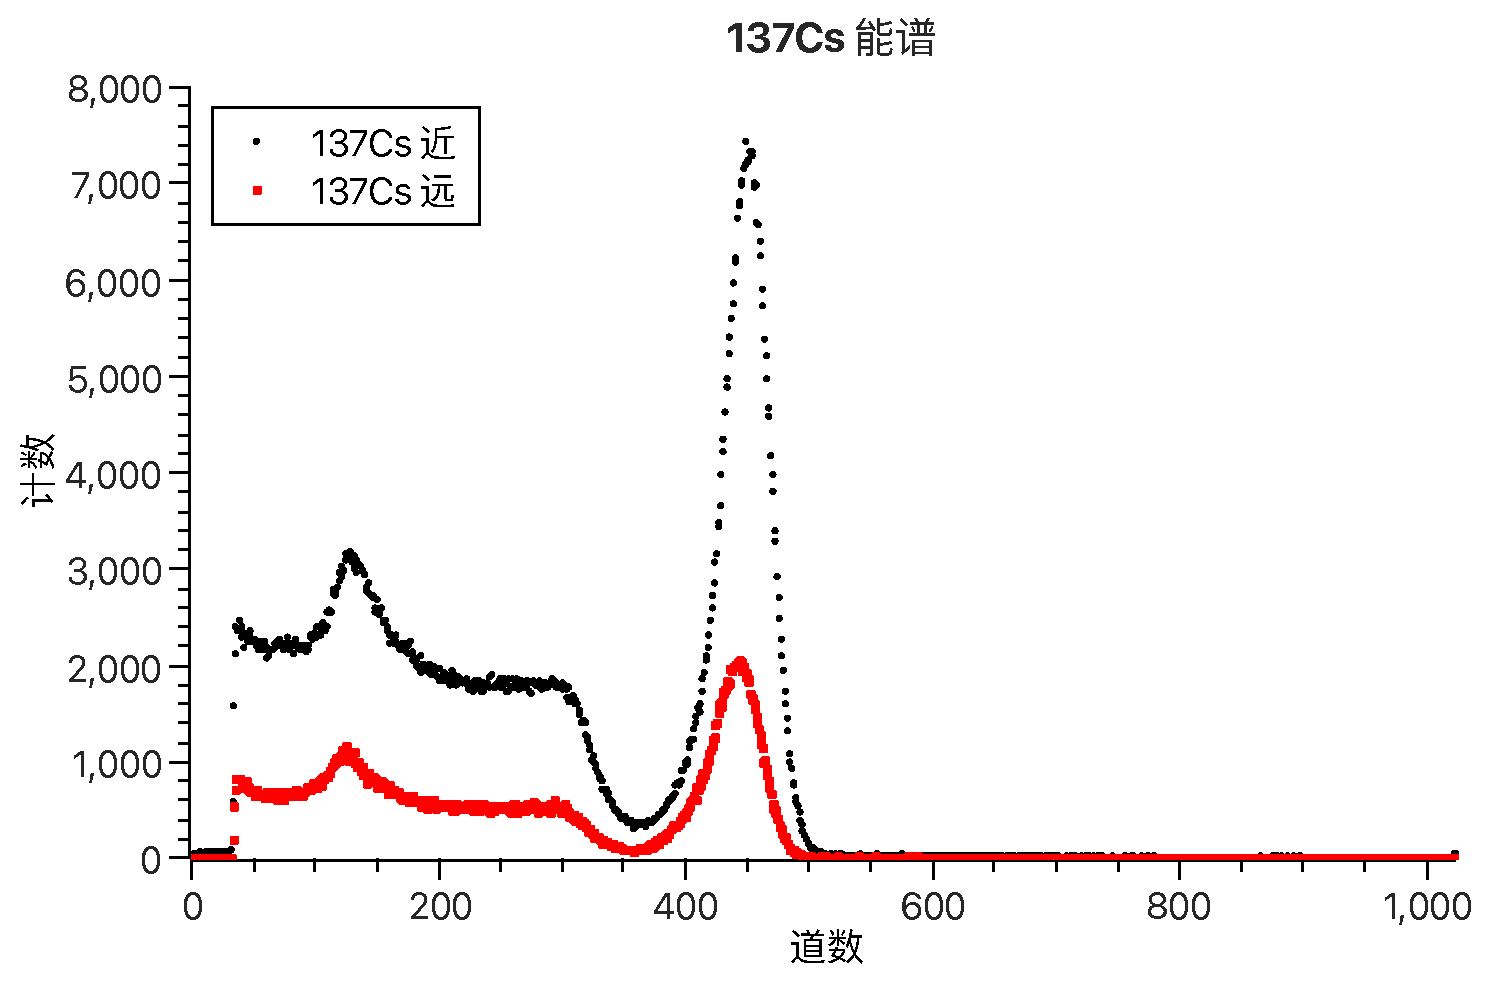
\includegraphics[width=0.5\textwidth]{./pic5.pdf}
        \caption{137Cs 能谱,其中黑点代表样品距离探头近,红点代表样品距离探头远}\label{fig:5}
    \end{figure}
    \begin{figure}[htbp]
        \centering
        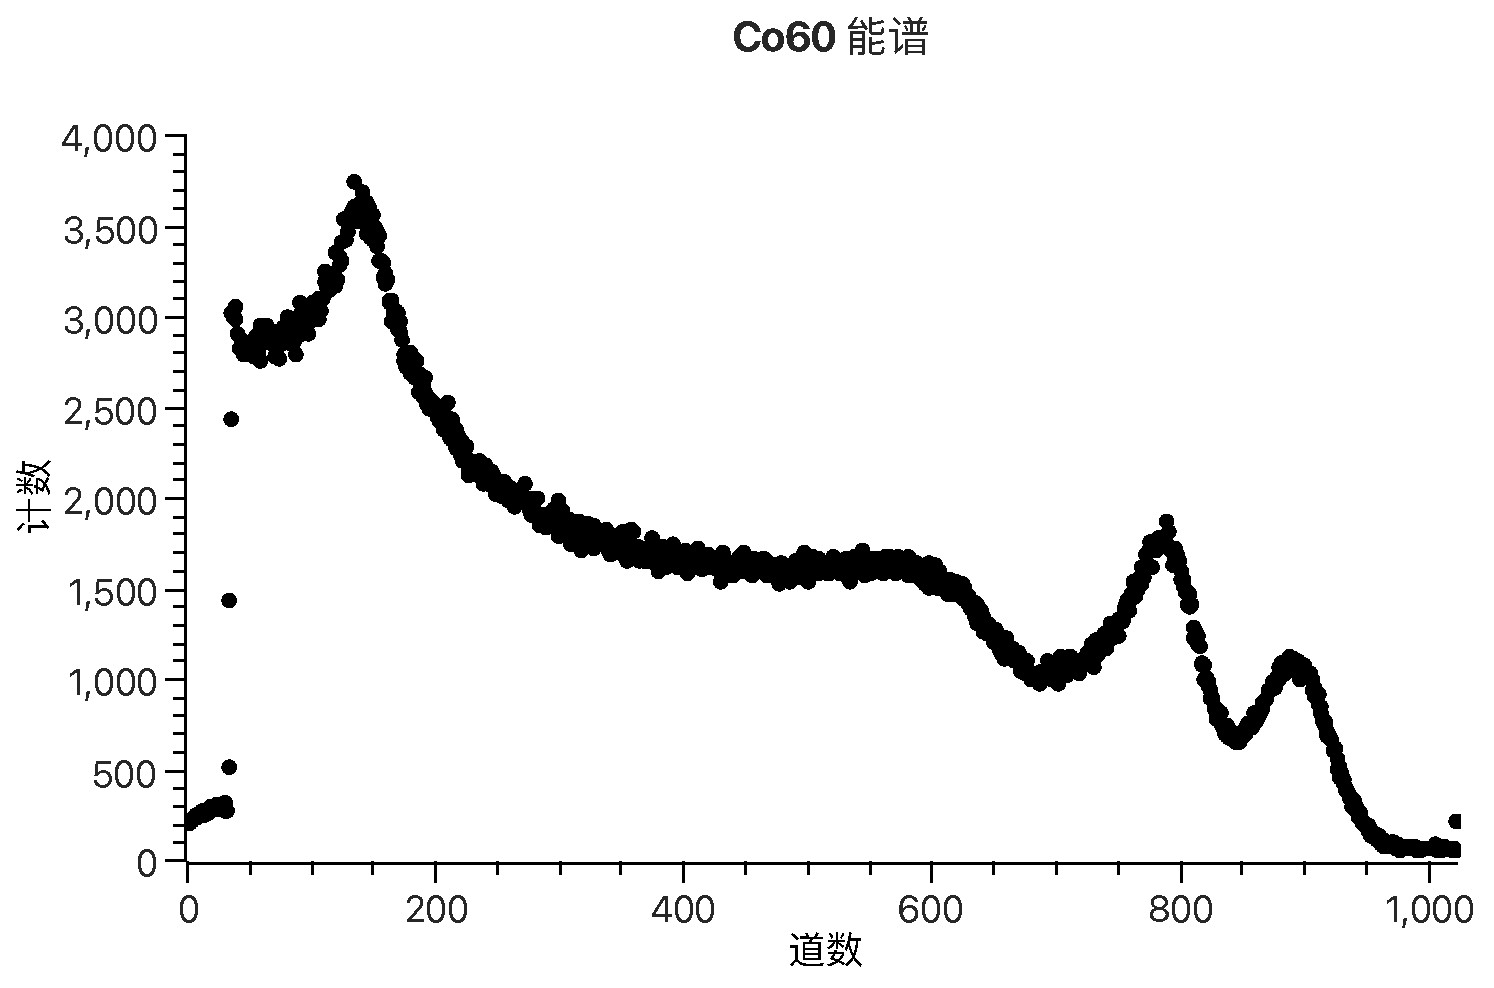
\includegraphics[width=0.5\textwidth]{./pic6.pdf}
        \caption{60Co 能谱}\label{fig:6}
    \end{figure}
    
    利用微机多道采集 137Cs 源、60Co 源的混合谱,采集定时取为 5 分钟,结果如\autoref{fig:7}。
    \begin{figure}[htbp]
        \centering
        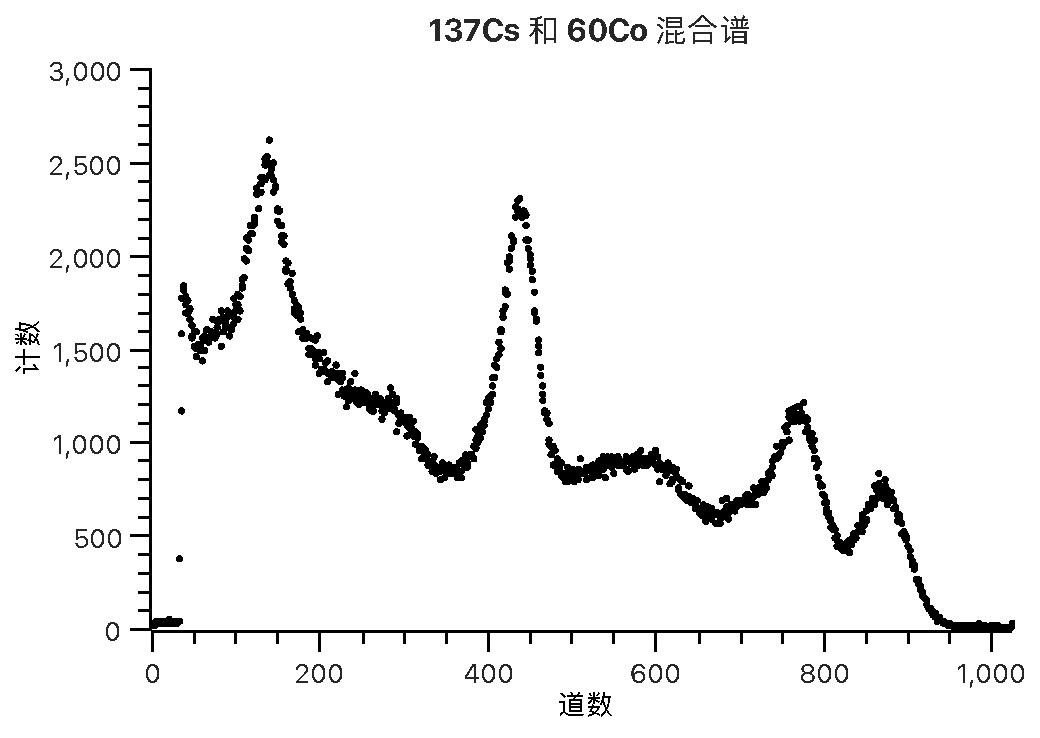
\includegraphics[width=0.6\textwidth]{./pic8.pdf}
        \caption{137Cs,60Co 混合能谱}\label{fig:7}
    \end{figure}
    可以从\autoref{fig:7}中看到137Cs和60Co的明显特征峰位,和预期的结果是相符的。
\section{结论}
    实验结合单道脉冲幅度分析器,利用 NaI 闪烁体探测器测量了 137Cs 源的 $\gamma$ 全
    能谱,以此探讨了 $\gamma$ 射线与物质相互作用的基本规律,分析了全能峰和反散射峰的由来。
    随后本实验结合 137Cs 和 60Co 的特征峰位对谱仪进行了能量刻度,
    并估计了谱仪的能量分辨率;在此基础上,利用多道分析器再次获得了 137Cs 源的全能谱,并测定了
    137Cs, 60Co 的混合能谱。
\begin{acknowledgments}
    感谢安刘攀老师的细致指导,关于闪烁体探测器的讲解和单道分析器的运作机制的讲解对本人带来了很大启发。
\end{acknowledgments}
\begin{thebibliography}{99}
    \bibitem{jindaishiyan} 吴思诚、荀坤. 近代实验物理[M]. 高等教育出版社, 2015.
\end{thebibliography}
\clearpage
\appendix
\section{思考题}
\subsection{若有一 $\gamma$ 射线源具有单一能量的 2MeV $\gamma$ 射线,试预言其谱形}
$\alpha = \frac{h\nu}{m_e c^2} = 3.914$,可以计算得到反散射峰的能量
$h\nu' = h\nu -E_{C \max} = h\nu \frac{1}{1+2\alpha} = 0.227\ \mathrm{MeV}$。

除了 $2$ MeV 全能峰和 $0.227$ MeV 反散射峰以外,由于 $\gamma$ 射线能量超过
$2m_e c^2$,会在 NaI 晶体中激发生成正负电子对,当它们在晶体中消耗尽能量后,会发生湮灭反应
放出一对 0.511 MeV 的光子。因此谱形中会出现三个特征峰 $0.227$ MeV, $0.511$ MeV, $2$ MeV,
且全能峰左侧会有一个平台,它来自康普顿电子的贡献和正负电子的贡献。
\end{document}